\ieeesection[SOFTWARE MODULES DESIGN]{SOFTWARE MODULES DESIGN}
\label{sec:software}

\textcolor{gray}{\rule{\linewidth}{3pt}}


\subsection{Architecture Overview}
\label{sec:arch_overview}
The software subsystem of CourtSweeper operates primarily on the NVIDIA Jetson Orin NX edge computing unit, utilizing a multi-threaded pipeline designed for high-throughput and low-latency operation. The architecture integrates heterogenous sensory inputs—comprising the high-definition DJI camera stream and 2D LiDAR range data—to establish full situational awareness.

\begin{figure}[htbp]
  \centering
  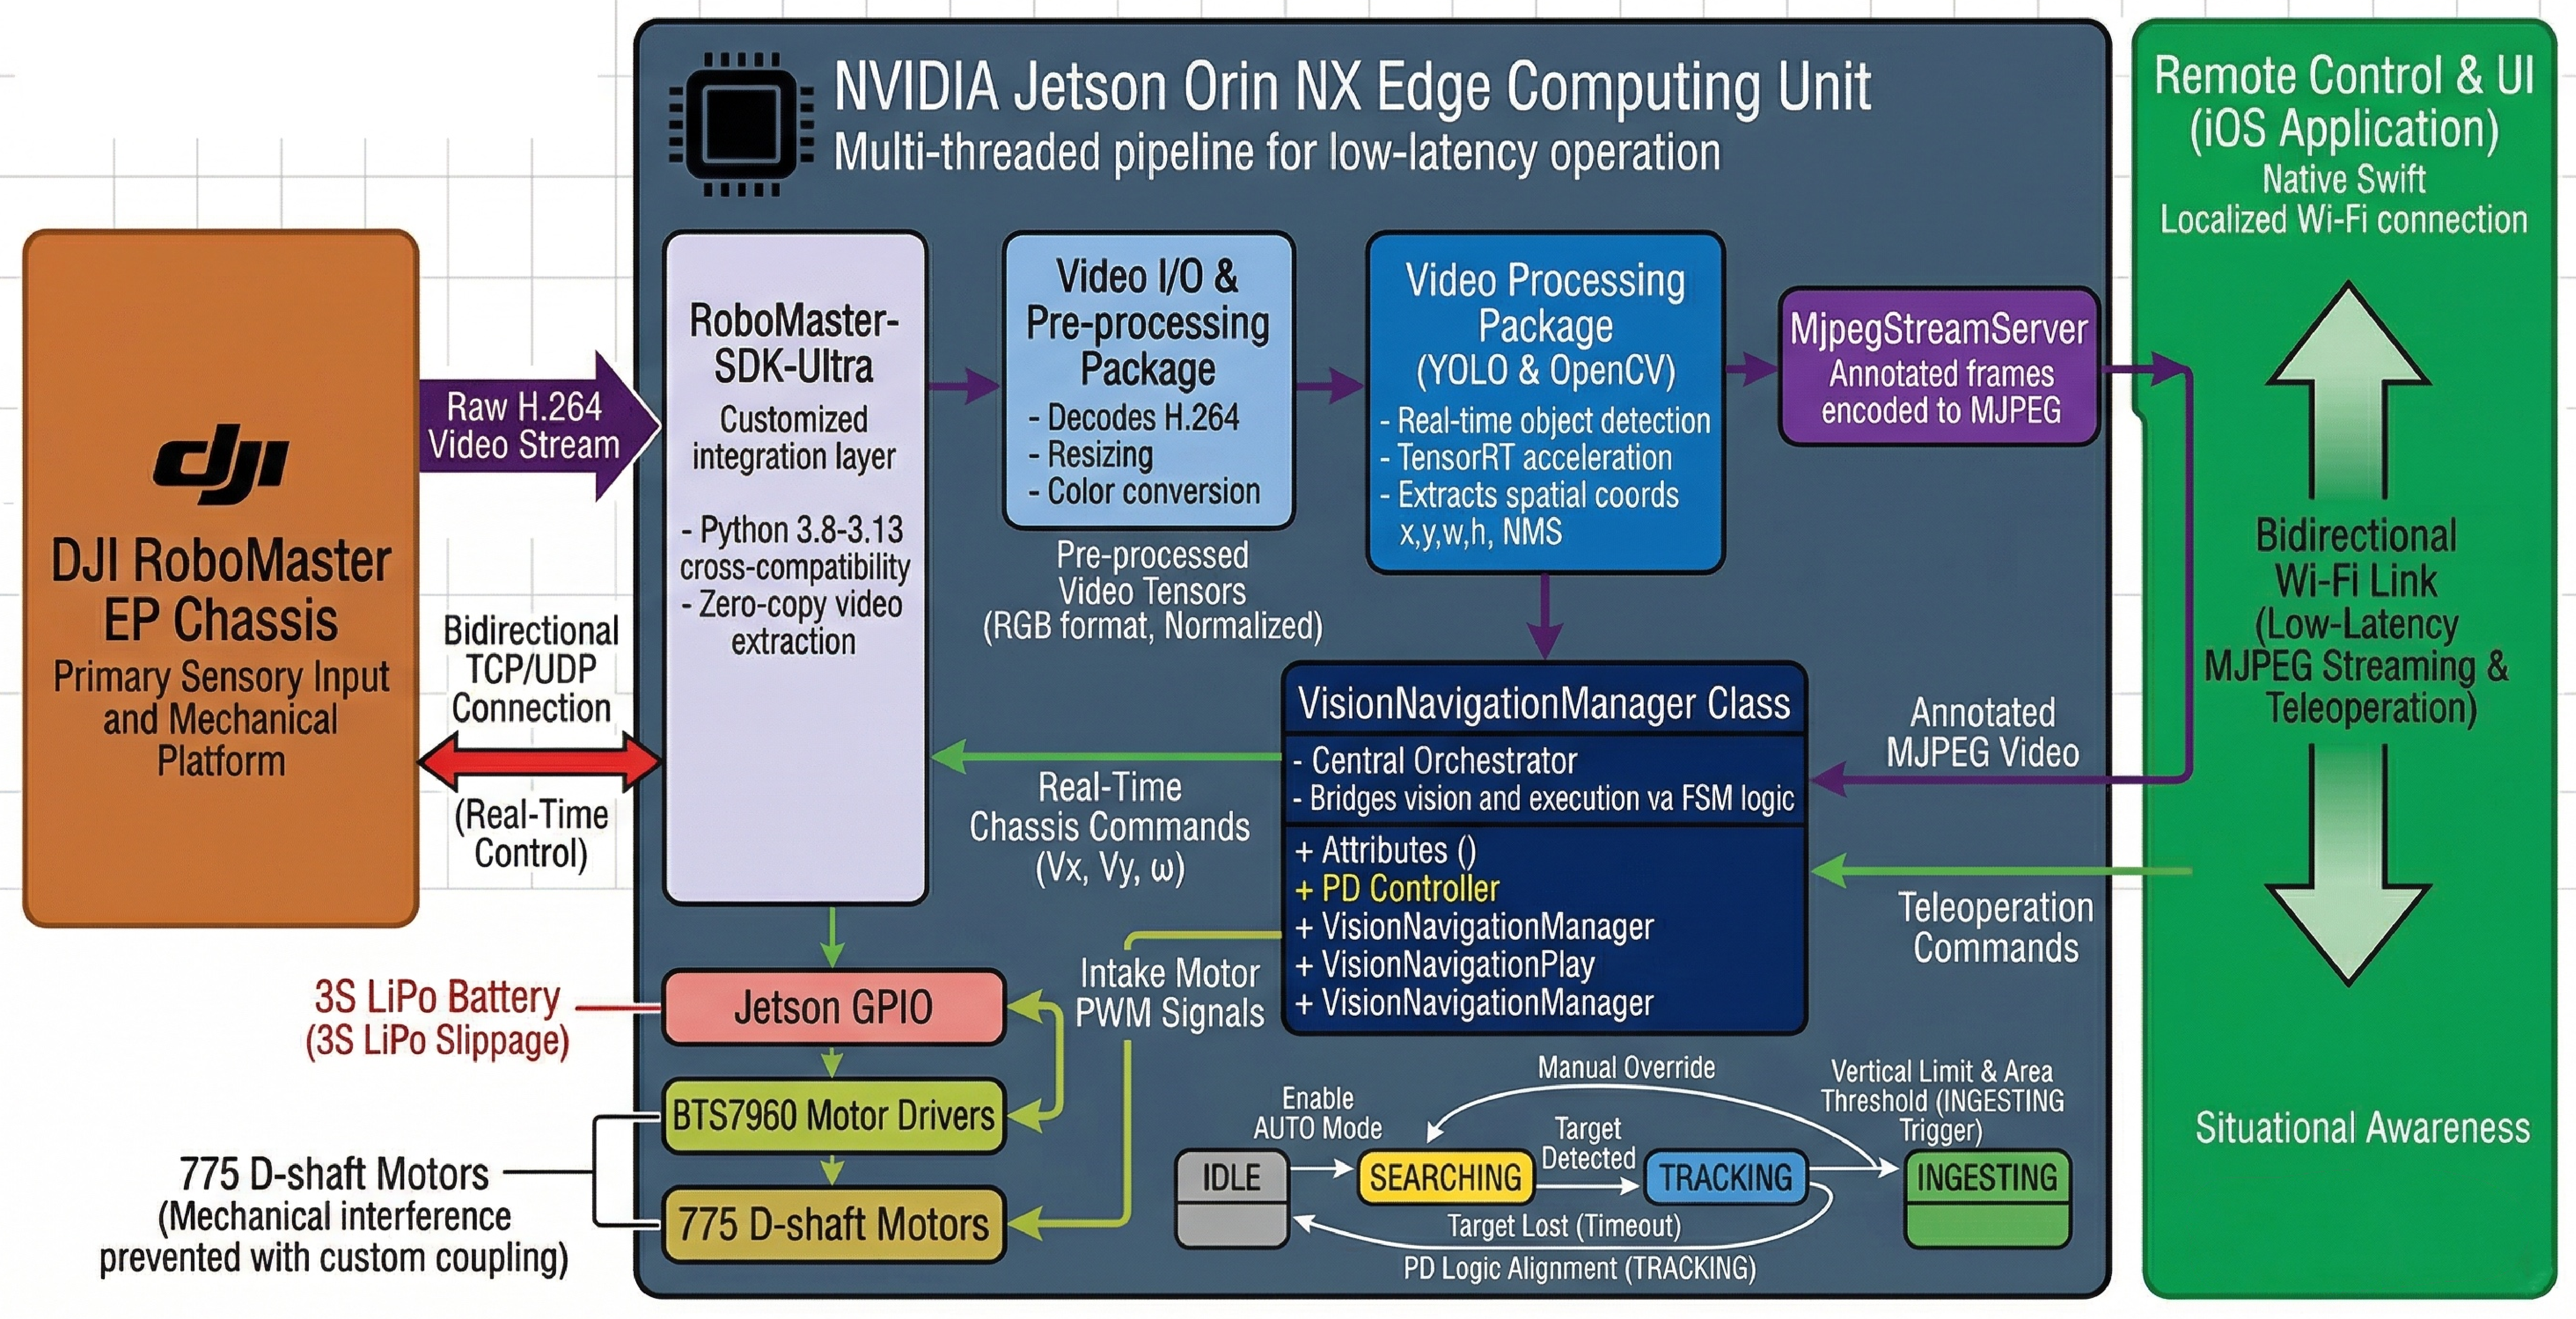
\includegraphics[width=0.9\textwidth]{figures/fig_software_overview.pdf}
  \caption{Detailed comprehensive diagram of the CourtSweeper software subsystem architecture, integrating visual perception and SLAM-based navigation pipelines.}
  \label{fig_software_overview}
\end{figure}

The core logic bridges these sensory inputs with the mechanical outputs (Mecanum chassis navigation and 775 motor actuation) through an advanced decision-making engine. This engine combines real-time SLAM (Simultaneous Localization and Mapping), heuristic workspace gridding, complete coverage path planning, and deep learning-based object detection, all governed by a robust Finite State Machine (FSM).


\subsubsection{Chassis Navigation \& DJI SDK Integration}
\label{sec:dji-sdk}
To interface with the mobile platform, the system implements the \textbf{RoboMaster-SDK-Ultra}, a customized integration layer offering native cross-compatibility across Python 3.8 $\sim$ 3.13. This allows DJI hardware drivers to coexist in the same execution environment as modern YOLO, OpenCV, and ROS-based SLAM pipelines, circumvents severe Inter-Process Communication (IPC) overhead when transferring large data matrices.

Operationally, this unified SDK manages a high-speed connection over the local network. It directly extracts the raw H.264 video stream from the integrated camera for zero-copy visual processing, while concurrently transmitting translational ($V_x, V_y$) and rotational ($\omega$) velocity commands back to the holonomic drive system based on calculated global paths or local reactive maneuvers.

\subsubsection{SLAM \& LiDAR Localization Package}
\label{sec:slam}
To provide the robot with precise spatial awareness, this package interfaces with the LiDAR via USB-serial. It implements a robust SLAM algorithm accelerated by the Jetson's GPU to process scan matching in real-time. This module is responsible for:
\begin{itemize}
  \item \textbf{Map Generation:} Constructing a 2D occupancy grid map of the surrounding environment during the initial setup phase.
  \item \textbf{Real-time Localization:} Providing continuous, high-frequency estimates of the robot's pose $(x, y, \theta)$ within the generated map by fusing LiDAR odometry and chassis wheel odometry data.
\end{itemize}

\subsubsection{Workspace Gridding \& Calibration Package}
\label{sec:gridding}
This module is utilized during system initialization to define the operational boundaries.
\begin{itemize}
  \item \textbf{Court Calibration:} The operator manually drives the robot along the perimeter of the tennis court playing area. The package records these pose boundaries within the SLAM map to isolate the sweeping workspace.
  \item \textbf{Grid Discretization:} The calibrated workspace is discretized into a uniform grid map. Each grid cell dimensions correspond to the sweeping width of the intake mechanism. Cells are classified as occupied (by static obstacles), traversable, cleared, or containing a target (projected from visual data).
\end{itemize}

\subsubsection{Coverage Path Planning Package}
\label{sec:path-planning}
This package is the core efficiency optimizer. In the absence of visually detected tennis balls, it ensures the entire traversable court area is swept systematically.
\begin{itemize}
  \item \textbf{Global Planning:} Utilizing algorithms such as A* or Spanning Tree Coverage, it generates an optimal coverage path through all traversable grid cells to minimize sweeping time and redundant traversal.
  \item \textbf{Local Planning \& Replenishment:} If visual processing detects a ball, the global coverage path is paused. After ball ingestion, the planner calculates a local trajectory back to the last paused waypoint on the global coverage path to resume systematic sweeping.
\end{itemize}

\subsubsection{Video I/O \& Pre-processing Package}
\label{sec:preprocessing}
Before AI inference, the raw H.264 video feed is decoded into discrete frame matrices. The pre-processing pipeline scales the HD frames to specified YOLO input dimensions and converts color spaces to RGB, normalizing pixel values to a $[0, 1]$ range for optimized neural network ingestion.

\subsubsection{Video Processing Package (YOLO \& OpenCV)}
\label{sec:video-processing}
Utilizing the YOLO architecture accelerated by TensorRT, this module performs real-time object detection to identify tennis balls. OpenCV functions extract the spatial coordinates of the bounding box $(x, y, width, height)$ and calculate the target centroid. 

Crucially, by utilizing the current robot pose from the SLAM package and known camera intrinsic parameters, this module projects the image-plane coordinates onto the ground plane to estimate the ball's $(x, y)$ location in the global map, updating the target status of specific grid cells.

\subsubsection{FSM-Based Event Recognition \& Control Package}
\label{sec:event-recognition}
The robot's behavioral logic is strictly governed by a Finite State Machine (FSM), decoupling perception from mechanical actuation. The optimized state transitions are as follows:
\begin{itemize}
  \item \textbf{State 0 - IDLE:} Awaiting commands. Manual teleoperation via iOS UI overrides all behaviors. Court calibration is performed in this state.
  \item \textbf{State 1 - SEARCHING (Optimized Coverage):} If no ball is visuals detected, the FSM enters searching state. Instead of random patrol, the chassis follows the pre-generated \textbf{Complete Coverage Path}. The system continuously ticks off grid cells as "cleared" upon traversal.
  \item \textbf{State 2 - TRACKING (Target Alignment):} Upon visual detection, FSM transitions to Tracking. Global path following is paused. A PD controller uses the camera centroid offset for rapid alignment, while a local planner drives the chassis toward the projected map coordinates of the ball.
  \item \textbf{State 3 - INGESTING (Intake Trigger):} As defined previously, triggered by bounding box area thresholds indicating physical contact. Motors activate via PWM. Upon successful ingestion, the corresponding grid cell is marked as "cleared," and the FSM transitions back to SEARCHING, utilizing the CPP package to return to the paused coverage path.
\end{itemize}


\subsection{Class Design}
\label{sec:class-design}

\paragraph{CourtNavigationManager Class Description}

To support the integrated SLAM and Planning pipelines, the central orchestrator is upgraded to the \texttt{CourtNavigationManager}. It bridges visual perception, spatial mapping, gridding, and path planning modules.

\begin{table}[H]
  \footnotesize
  \centering
  \renewcommand{\arraystretch}{1.3}
  \begin{tabularx}{\textwidth}{|l|X|}
    \hline
    \rowcolor[RGB]{220,220,220} \textbf{Attribute} & \textbf{Description} \\ \hline
    Class Name & \texttt{CourtNavigationManager} \\ \hline
    Aggregated Classes & \texttt{YoloDetector}, \texttt{SlamLocalizer}, \texttt{GridMapHandler}, \texttt{CoveragePathPlanner}, \texttt{DjiChassisController}, \texttt{MotorPwmDriver} \\ \hline
    Associated Classes & \texttt{MjpegStreamServer}, \texttt{RosBridgeServer} (for LiDAR data) \\ \hline
    Data Members & 
    \textbullet~ \texttt{current\_state}: Enum (IDLE, CALIBRATING, SEARCHING, TRACKING, INGESTING). \newline
    \textbullet~ \texttt{robot\_pose\_global}: Pose $(x, y, \theta)$ provided by \texttt{SlamLocalizer}. \newline
    \textbullet~ \texttt{discretized\_grid}: 2D Array/Structure managing cell states (Occupied, Swept, Ball). \newline
    \textbullet~ \texttt{global\_coverage\_path}: List of Waypoints to ensure 100\% coverage. \\ \hline
    Member Functions & 
    \textbullet~ \texttt{update\_master\_state()}: High-level FSM logic switching based on vision, path progress, and grid status. \newline
    \textbullet~ \texttt{calibrate\_court\_perimeter()}: Records boundary poses during manual driving to define grid limits. \newline
    \textbullet~ \texttt{generate\_gridded\_workspace()}: Discretizes calibrated area and calls \texttt{CoveragePathPlanner} for the initial path. \newline
    \textbullet~ \texttt{compute\_navigation\_command()}: In SEARCHING, computes commands to follow the coverage path. In TRACKING, switches to PD-based visual servoing and projected coordinate driving. \\ \hline
    Processing & Operates in a dedicated high-priority thread. It fuses pose data and vision data to update the grid map, executes the FSM, dispatches velocity commands to the DJI SDK, and triggers intake motors. \\ \hline
  \end{tabularx}
\end{table}